\chapter{Incertezza}

\section{Introduzione}

\qs{}{
  Indichiamo con $A_t$ il piano che ci fa partire per l'aeroporto $t$ minuti prima del decollo. Come stabilire se $A_t$ ci porterà in aeroporto per tempo?}

\paragraph{Problemi:}

\begin{itemize}
  \item Osservabilità parziale (stato delle strade, traffico, etc.). 
  \item Osservazioni imprecise (notizie traffico/meteo inesatte). 
  \item Incertezza sul risultato delle azioni (la macchina non parte). 
  \item Difficile modellare un sistema nel suo complesso.
\end{itemize}

\paragraph{Se si sceglie un approccio puramente logico:}

\begin{itemize}
  \item Si rischia di prendere decisioni errate. 
  \item Si hanno conclusioni \fancyglitter{troppo deboli} per il decision making.
\end{itemize}

\paragraph{Limiti della logica del primordine:}

\begin{itemize}
  \item \fancyglitter{Pigrizia:} elencare un insieme completo di premesse/conseguenze richiede troppo lavoro, le regole diventano difficili da comprendere e utilizzare.
  \item \fancyglitter{Ignoranza teorica:} non conosciamo tutto. 
  \item \fancyglitter{Ignoranza pratica:} anche se conosciamo tutto in generale potremmo avere lacune sul caso specifico.
\end{itemize}

\subsection{Probabilità}

\dfn{Probabilità}{
La probabilità fornisce uno strumento per riassumere l’incertezza che deriva da pigrizia e ignoranza. Si assegna una probabilità a una formula corrisponde al grado di credenza nella verità della formula.
}

\clm{}{}{
  \begin{itemize}
    \item Le credenze dipendono dalle prove. Tutti gli enunciati indicheranno sempre le prove alla base degli assegnamenti di probabilità. 
    \item Due casi:
      \begin{itemize}
        \item Probabilità a priori: in assenza di prove. 
        \item Probabilità a posteriori: dopo avere osservazioni.
      \end{itemize}
  \end{itemize}
}

\paragraph{Prendere decisioni razionali:}

\begin{itemize}
  \item Attribuiamo a $A_{90}$ probabilità $95\%$ di successo. 
  \item $A_{120}$ e $A_{1440}$ avranno probabilità anche maggiori ma sono necessariamente migliori?
  \item Per prendere \fancyglitter{decisioni razionali} un agente deve avere preferenza sugli esiti delle sue azioni. 
  \item La \fancyglitter{teoria dell'utilità} attribuisce a ogni esito un grado di utilità per l'agente e permette all'agente di ragionare su esiti alternativi. 
  \item Teoria delle decisioni = Teoria delle Probabilità + Teoria dell'Utilità.
\end{itemize}

\clm{Convenzioni sulla notazione}{}{
  \begin{itemize}
    \item \fancyglitter{Variabile casuale} si riferisce a una parte del mondo il cui stato è inizialmente sconosciuto. 
    \item Le probabilità sono associate a proposizioni del tipo $X = Val$ dove $X$ è la variabile casuale discreta e $val$ è un valore del suo dominio. 
    \item Con lettere minuscole $a, b, c$ si indica variabili casuali generiche. 
    \item Con lettere maiuscole si indicano variabili casuali di un dominio specifico. 
  \end{itemize}
}


\paragraph{Assiomi delle probabilità:}

\begin{itemize}
  \item Per qualsiasi proposizione $a$ e $b$: 
    \begin{enumerate}
      \item $0 \leq P(a) \leq 1$
      \item $P(\text{true}) = 1$ \quad e \quad $P(\text{false}) = 0$
      \item $P(a \lor b) = P(a) + P(b) - P(a \land b)$
    \end{enumerate}
  \item Questi assiomi sono detti \fancyglitter{assiomi di Kolmogorov}.
  \item Motivazioni:
    \begin{itemize}
      \item L’uso degli assiomi nella rappresentazione di “gradi di belief” come probabilità garantisce razionalità e consistenza delle decisioni.
      \item I CF sono un esempio di gradi di belief che non soddisfano gli assiomi: trade-off tra poter ragionare con regole di buon senso e complessità computazionale.
    \end{itemize}
\end{itemize}

\dfn{Evento Atomico}{
  Specifica completa dello stato del mondo. È un assegnamento di valori a tutte le variabili casuali. 
}

\paragraph{Proprietà degli eventi atomici:}

\begin{itemize}
  \item Sono mutuamente esclusivi. 
  \item L'insieme di tutti gli eventi atomici descrive la verità o la falsità di qualsiasi proposizione (semplice o complessa). 
  \item Ogni proposizione è logicamente equivalente alla disgiunzione di tutti gli eventi atomici che ne implicano la verità. 
  \item In generale, dati $e(a)$ insieme degli eventi atomici dove $a$ è vera, $$P(a) = \displaystyle\sum_{e_i \in e(a)} P(e_i)$$ 
\end{itemize}

\subsection{Probabilità a Priori e a Posteriori}

\dfn{Probabilità a Priori}{
  È il grafo di credenza in una proposizione $a$ in \fancyglitter{assenza di ogni altra informazione}.
}

\cor{Distribuzione di Probabilità}{
  La distribuzione di probabilità a priori è un vettore di valori di probabilità: uno per ogni valore del dominio della variabile casuale considerata. 
}

\nt{I valori sono normalizzati in modo che la somma sia uguale a 1.}

\cor{Distribuzione di Probabilità Congiunta}{
  È una matrice che assegna un valore di probabilità a ogni possibile combinazione di valori delle variabili considerate. 
}

\nt{La distribuzione di probabilità congiunta è completa se costruita su tutte le variabili del dominio.}

\dfn{Probabilità Condizionate (a Posteriori)}{
  $P(a|b)$ è la probabilità di $a$ quando tutto ciò che sappiamo è $b$: 
  $$P(a|b) = \displaystyle\frac{P(a \land b)}{P(b)}$$
  quando $P(b) \not = 0$.
}

\cor{Regola del Prodotto}{
  $$P(a \land b) = P(a|b)*P(b) = P(b|a)*P(a)$$
}

\nt{Le probabilità condizionate non sono implicazioni logiche con incertezze. Inoltre le probabilità condizionate non sono monotone.}

\subsection{Inferenze con Distribuzioni di Congiunzione Complete}

\dfn{Inferenza Probabilistica}{
  Calcolo delle probabilità a posteriori poste come interrogazioni (query) partendo dalle prove osservate.
}

\cor{Regola del Condizionamento}{
  $$P(Y) = \displaystyle\sum_{z} P(Y|z)*P(z)$$
}

\nt{Nella maggior parte dei casi è interessante calcolare la probabilità condizionata di qualche variabile, avendo a disposizione altre variabili come prova. }

\cor{Inferenza Generale}{
  $$P(X|e) = \alpha P(X, e) = \alpha \displaystyle\sum_{y} P(X, e, y)$$

  In cui:
  \begin{itemize}
    \item E: variabili di evidenza. 
    \item Y: variabili nascoste. 
    \item X: variabili di query.
  \end{itemize}
}

\paragraph{Questa procedura ha due svantaggi:}

\begin{itemize}
  \item È computazionalmente costosa. 
  \item Costruire la distribuzione congiunta completa non è sempre possibile nei casi reali.
\end{itemize}

\section{Regola di Bayes}

\dfn{Indipendenza}{
  $a$ e $b$ sono indipendenti tra di loro se e solo se $P(a|b) = P(a)$ o $P(b|a) = P(b)$ o $P(a \land b) = P(a) * P(b)$.
}

\nt{Nei domini reali l'Indipendenza assoluta è rara.}

\dfn{Regola di Bayes}{
  $$P(b|a) = \displaystyle\frac{P(a|b) * P(b)}{P(a)}$$
}

\nt{Il teorema di Bayes può essere generalizzato.}

\dfn{Regola di Bayes e Condizionamento all'Evidenza}{
  $$P(Y|X, e) = \displaystyle\frac{P(X|Y, e) * P(Y|e)}{P(X|e)}$$
dove $e$ è un vettore di valori alle variabili di prova.
}

\subsection{Modelli di Bayes}

\dfn{Modello di Bayes Ingenuo}{
  $$P(\text{Causa, Effetto$_1$, \dots, Effetto$_2$}) = P(\text{Causa}) \prod_i P(\text{Effetto$_i |$ Causa})$$
}

\nt{L'ingenuità sta nel fatto che si assume che gli $n$ effetti siano tra loro indipendenti, ma nei casi reali spesso non è così.}

\dfn{Indipendenza Condizionale}{
  L'indipendenza condizionale di $X$ e $Y$ data $Z$ vale se e solo se: 

  $$P(X, Y|Z) = P(X|Z)*P(Y|Z)$$

}

\paragraph{Se l'indipendenza condizionale vale allora:}

\begin{itemize}
  \item $P(X|Y, Z) = P(X|Z)$
  \item $P(Y|X, Z) = P(Y|Z)$
\end{itemize}

\dfn{Belief Networks}{
È una rappresentazione grafica di asserzioni di indipendenze condizionali. Fornisce una specifica concisa di qualsiasi distribuzione congiunta completa. È un grafo:
\begin{itemize}
  \item Un nodo per ogni variabile casuale. 
  \item Diretto e privo di cicli. 
  \item Un arco da $X$ a $Y$ implica che $X$ è un genitore di $Y$ e ha influenza diretta. 
  \item Ogni nodo $X_i$ è associato a una distribuzione condizionale di $X_i$ dati i suoi genitori $P(X_i | \text{parents}(X_i))$. 
  \item In generale la Tabella di Probabilità Condizionali (CPT\footnote{Non TCP.}) di una variabile booleana con $k$ genitori booleani contiene $2^k$ righe.
\end{itemize}
}

\nt{La topologia della rete specifica le condizioni di indipendenza e definisce implicitamente la distribuzione congiunta completa di tutte le variabili casuali.}

\cor{Compattezza}{
  Una CPT per una variabile booleana $X_i$ con $k$ genitori booleani ha $2^k$ righe per tutte le possibili combinazioni di valori dei genitori. Ogni riga contiene un valore $p$ per $X_i = true$, se ogni variabile ha non più di $k$ genitori la rete completa richiede $O(n*2^k)$. Dato che in generale $k << n$ il numero di valori necessari cresce linearmente in $n$ contro $O(2^n)$ della distribuzione completa congiunta.
}

\dfn{Semantica Globale}{
  Stabilisce come la struttura (sintassi) della BN corrisponde a una distribuzione congiunta delle variabili. La distribuzione completa congiunta può essere riscritta come il prodotto delle distribuzioni condizionali locali:

$$P(X_1,\dots, X_2) = \prod_{i=1}^n P(X_i | \text{Parents}(X_i))$$

}

\nt{Questa semantica è equivalente a una semantica local.}

\dfn{Semantica Locale}{
  Ogni nodo è condizionalmente indipendente dai suo non-discendenti dati i suoi genitori.
}

\cor{Markov Blanket}{
  Ogni nodo è condizionalmente indipendente da tutti gli altri nodi di una rete data la sua coperta di Markov: genitori, discendenti e genitori dei discendenti.
}

\paragraph{Costruire una BN:}

\begin{itemize}
  \item Si deve fare attenzione all'ordine con cui i nodi sono aggiunti nella rete stessa. 
  \item \fancyglitter{Chain rule:}
    \begin{align*}
\mathbb{P}(X_1, \ldots, X_n) 
&= \mathbb{P}(X_1 \mid X_2, \ldots, X_n) \mathbb{P}(X_2, \ldots, X_n) \\
&= \mathbb{P}(X_1 \mid X_2, \ldots, X_n) \mathbb{P}(X_2 \mid X_3, \ldots, X_n) \mathbb{P}(X_3, \ldots, X_n) \\
&= \cdots \\
&= \prod_{i=1}^{n} \mathbb{P}(X_i \mid X_{i+1}, \ldots, X_n)
\end{align*}
\item La chain rule è uguale alla semantica globale purché $\text{Parents}(X_i) \subseteq \{X_{i+1},\dots, X_n\}$
\end{itemize}

\nt{Una rete rispetta la semantica globale delle BN solo se per ogni nodo $X_i$ esso è condizionalmente indipendente da ogni altro suo predecessore nel'’ordine dei nodi, dati i suoi genitori.}

\paragraph{Strategia di costruzione:}

\begin{enumerate}
  \item Si sceglie un ordinamento delle variabili $X_n, \dots, X_1$.
  \item Per ogni $i$ da $n$ fino a 1:
    \begin{enumerate}
      \item Si aggiunge $X_i$ alla rete. 
      \item Si scelgono genitori da $X_{i+1},\dots, x_i$ tali che $P(X_i|\text{Parents}(X_i)) = P(X_i|X{i+1},\dots, X_n)$
    \end{enumerate}
\end{enumerate}

\section{Inferenza con le Reti Bayesiane}

\paragraph{Data una rete definita su un insieme di variabili U, occorre distinguere tra:}

\begin{itemize}
  \item Variabili di evidenza E. 
  \item Variabili di query X. 
  \item Variabili nascoste Y = U - E - X.
\end{itemize}

\dfn{Procedura di Inferenza Generale}{
  \[
\mathbb{P}(X \mid \mathbf{e}) = \alpha \, \mathbb{P}(X, \mathbf{e}) = \alpha \sum_{y} \mathbb{P}(X, \mathbf{e}, y)
\]

}

\paragraph{Algoritmo di eliminazione delle variabili:}

\begin{itemize}
  \item La procedura di calcolo può essere migliorata evitando di ripetere più volte gli stessi calcoli. 
  \item Programmazione dinamica: svolto un calcolo ne ricordo il risultato per uso futuro. 
  \item Una possibile implementazione è proprio questo algoritmo.
\end{itemize}

\dfn{Algoritmo di Eliminazione delle Variabili}{
  Partendo dalla formulazione di una query che esplicità tutte le sommatorie nascoste si individuano i fattori della formula e si valuta la formula da destra verso sinistra svolgendo due operazioni fondamentali sui fattori:
  \begin{itemize}
    \item Dot product tra fattori. 
    \item Eliminazione di una variabile per summing out.
  \end{itemize}
}

\cor{Dot Product}{
  Dati due fattori $f$ e $g$ il loro prodotto puntuale produce un nuovo fattore $h$ le cui variabili sono date dall'unione delle variabili dei fattori di partenza.
}

\nt{La complessità spaziale e temporale dell'algoritmo di eliminazione nasce proprio da questa caratteristica.}

\begin{figure}[h]
    \centering
    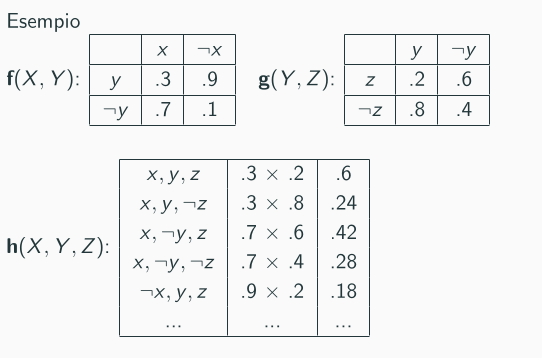
\includegraphics[scale=0.55]{03/dot.png}
    \caption{Esempio di dot product.}
\end{figure}

\dfn{Eliminazione per Summing Out}{
  Si elimina una variabile da un prodotto di fattori sommando le sottomatrici ottenute fissando la variabile a ognuno dei suoi valori.
}

\cor{Ottimizzazione - Safe Pruning}{
  Ogni fattore che non dipende dalla variabile da eliminare con summing out può essere portato fuori dalle sommatorie. Le matrici non sono moltiplicate fino a quando non dobbiamo eliminare una variabile di conseguenza si moltiplicano solo le matrici che contengono la variabile da eliminare.
}
\nt{Si può fare ancora meglio osservando che qualsiasi nodo foglia che non è né variabile di query né di evidenza può essere ignorata.}

\clm{}{}{
  \begin{itemize}
    \item La rimozione di un nodo foglia può dare origine a un altro nodo foglia a sua volta eliminabile. 
    \item In generale ogni variabile che non è un progenitore di una variabile di query o di evidenza è irrilevante per risolvere l'interrogazione (semantica locale).
  \end{itemize}
}

\cor{Ottimizzazione - Ordinamento delle Variabili}{
  L'ordinamento delle variabili ha un impatto sull'albero di parsificazione della formula e quindi sui fattori che vengono prodotti. Il risultato finale non dipende dall'ordinamento scelto, ma ordinamenti diversi producono fattori intermedi diversi. Più sono grandi questi fattori intermedi peggio è.
}
\nt{Si deve trovare l'ordinamento ottimale, tuttavia è un problema intrattabile.}
